\chapter{Umgesetzter Funktionsumfang}
In diesem Kapitel wird der aktuelle Funktionsumfang des Bots beschrieben und durch Bilder veranschaulicht.

Der Funktionsumfang besteht aus den folgenden Telegram-Befehlen:

\begin{description}
  \item[/start] \hfill \\
  Startet das Abonnement aller Nachrichten, welche aus Informationen des Schwarzen Bretts über die Studiengänge Informatik Bachelor, Medien- und Kommunikationsinformatik Bachelor, Informatik Master und die offiziellen Fakultätsnachrichten bestehen.

  Beim Erneuten Aufrufen von \emph{/start} wird der Nutzer darauf aufmerksam gemacht, dass er bereits angemeldet ist.
  \item[/stop] \hfill \\
  Beendet das Abonnement. Somit erhält der User ab sofort keine Nachrichten mehr. Es ist trotzdem weiterhin möglich \emph{/mensa} und \emph{/profs} zu benutzen.

  Beim Erneuten Aufrufen von \emph{/stop} wird der Nutzer darauf aufmerksam gemacht, dass er bereits abgemeldet ist.
  \newpage
  \item[/abo] \hfill \\
  Der User kann einzelne Nachrichtenkategorien an- und ababonnieren und so seine Auswahl personalisieren.

  Dabei werden kleine Notifications zur Bestätigung und Überprüfung der Eingabe am oberen Bildschirm der Telegram-App angezeigt. Als weitere Bestätigung werden die Button-Texte aktualisiert. \\
  Beispiel: \textbf{INFM abonnieren} wird zu \textbf{INFM abbestellen}

  \begin{figure}[!htb]
      \centering
      \caption{Blick auf die /abo-Funktionalität}
        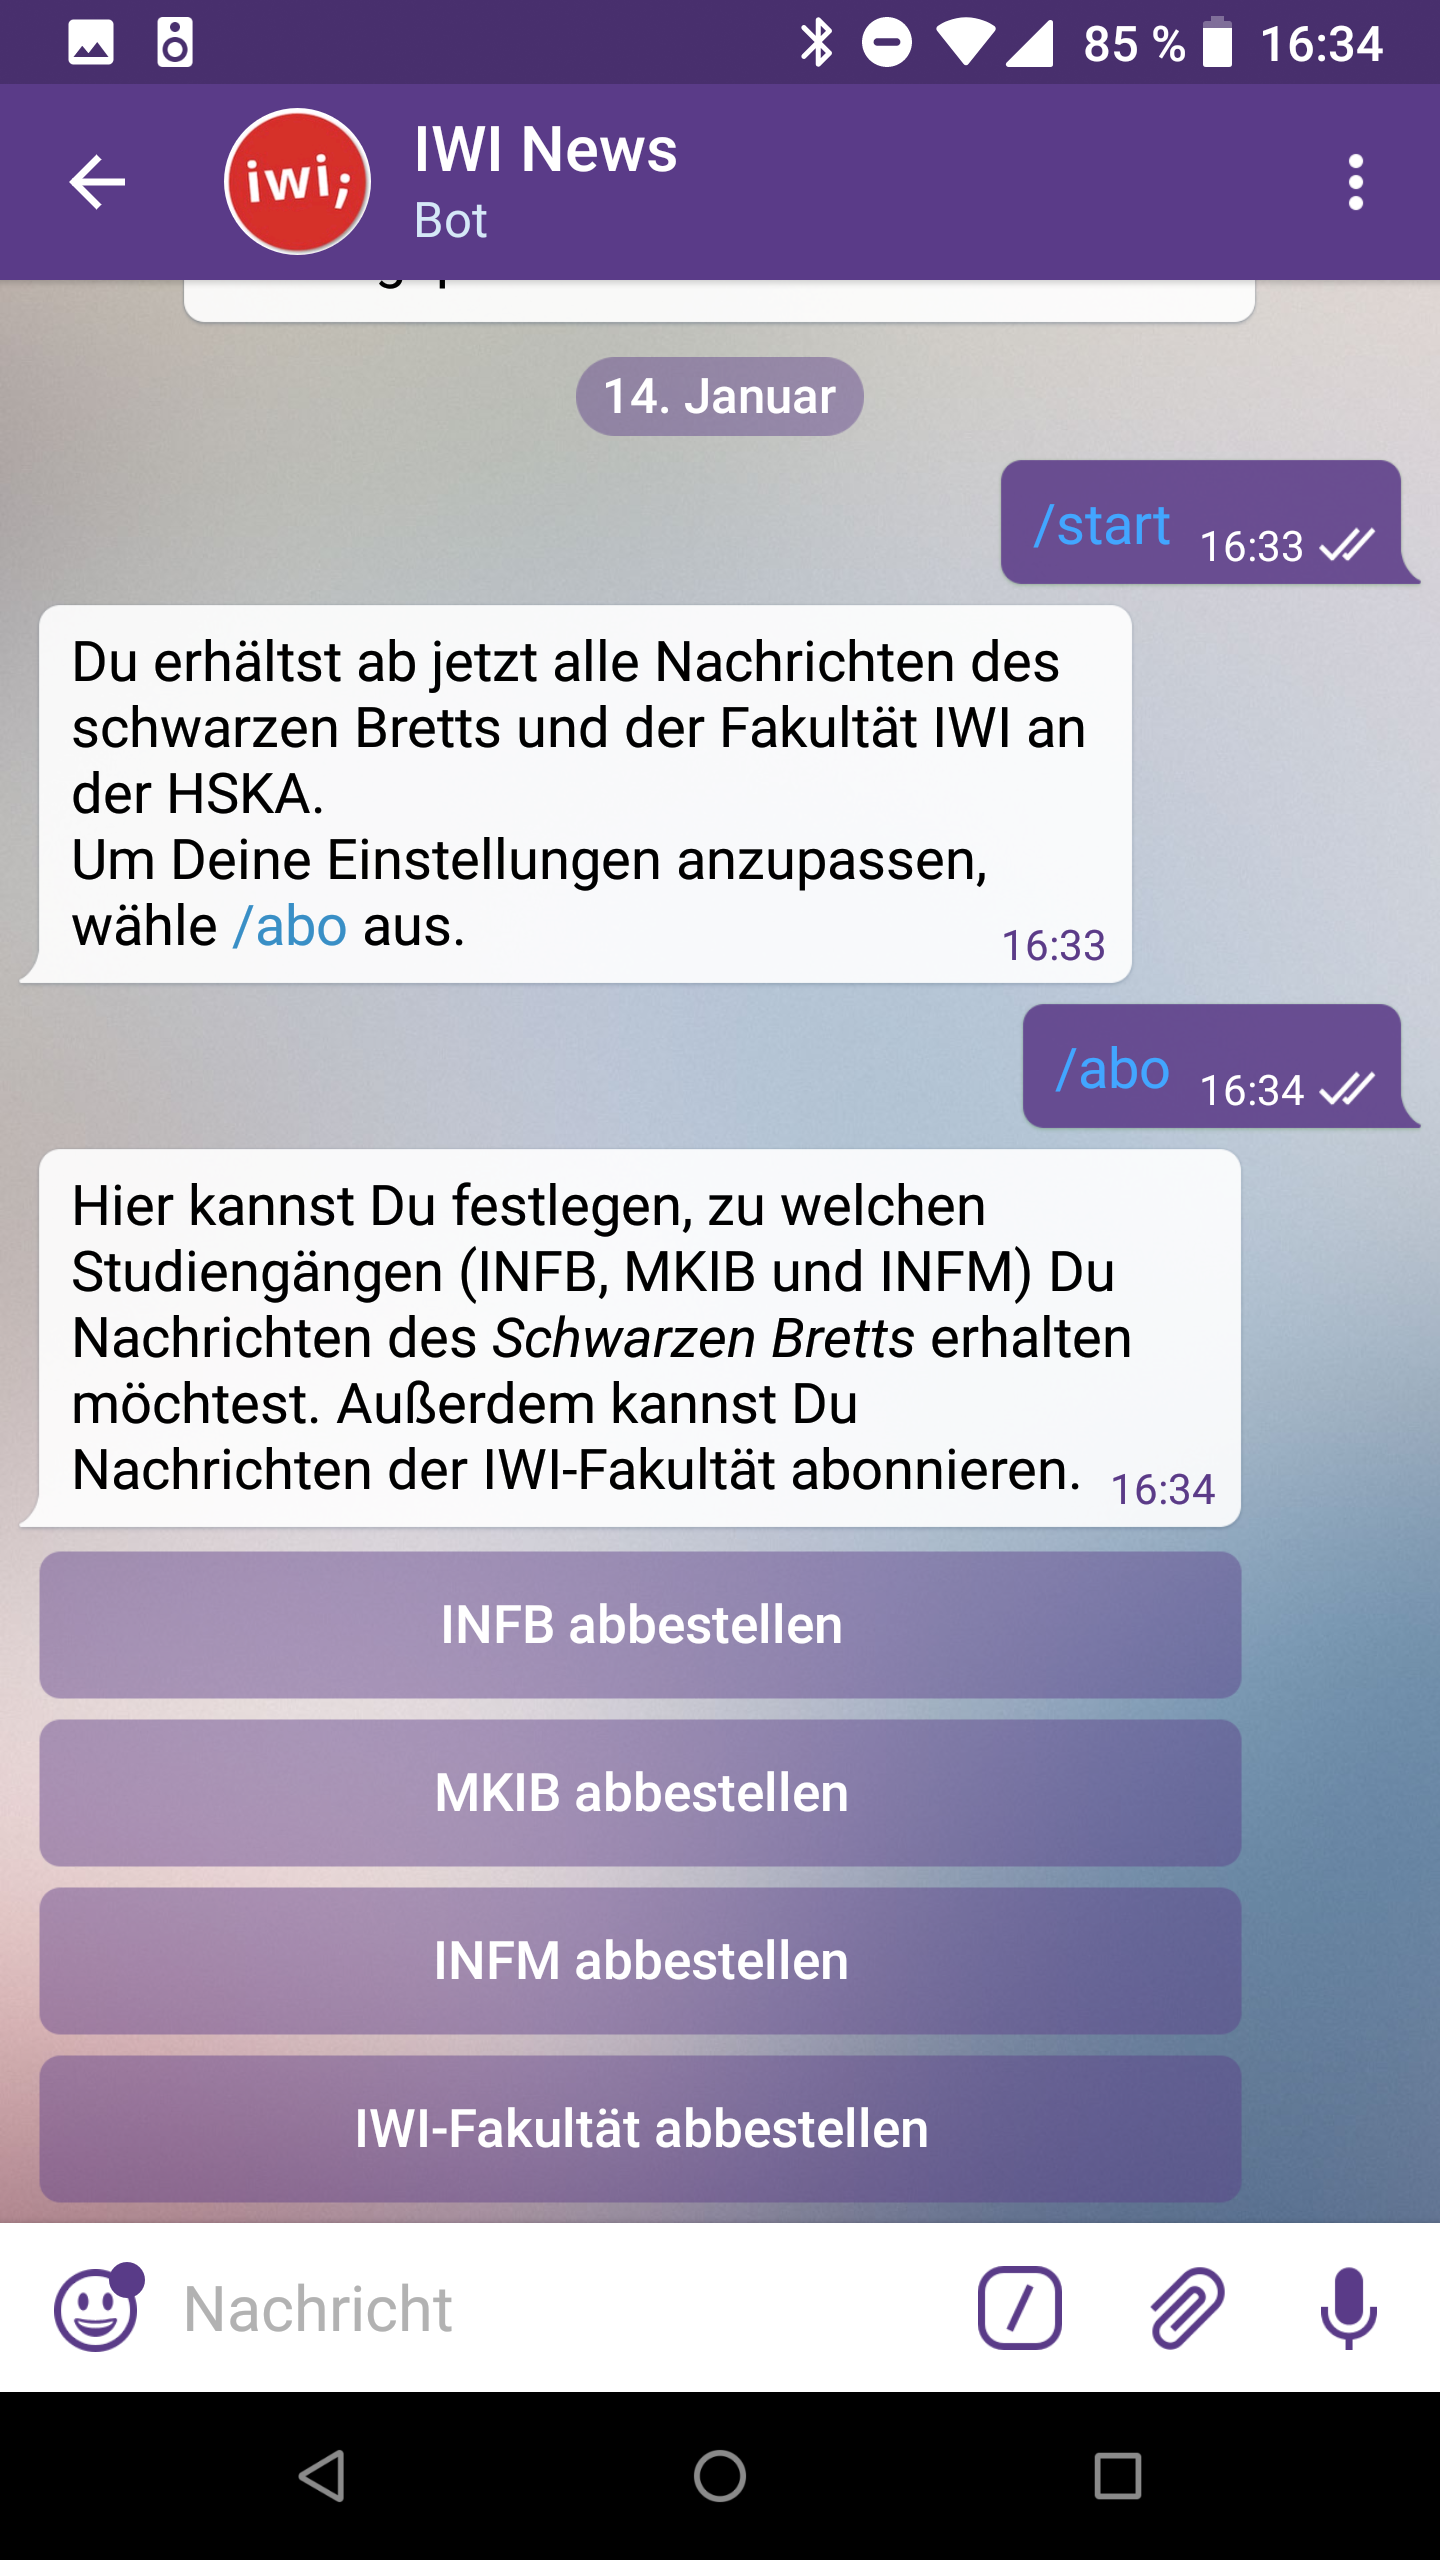
\includegraphics[width=0.4\linewidth]{BotAbo.png}
      \caption*{Quelle: Eigene Abbildung}
  \end{figure}

  \item[/mensa] \hfill \\
  Der User erhält die Möglichkeit, sich für die nächsten fünf Tage das Mensaangebot ausgeben zu lassen. Dabei wird das Wochenende ausgespart, da es dann kein Angebot gibt.

  \begin{figure}[!htb]
      \centering
      \caption{Blick auf die /mensa-Funktionalität}
        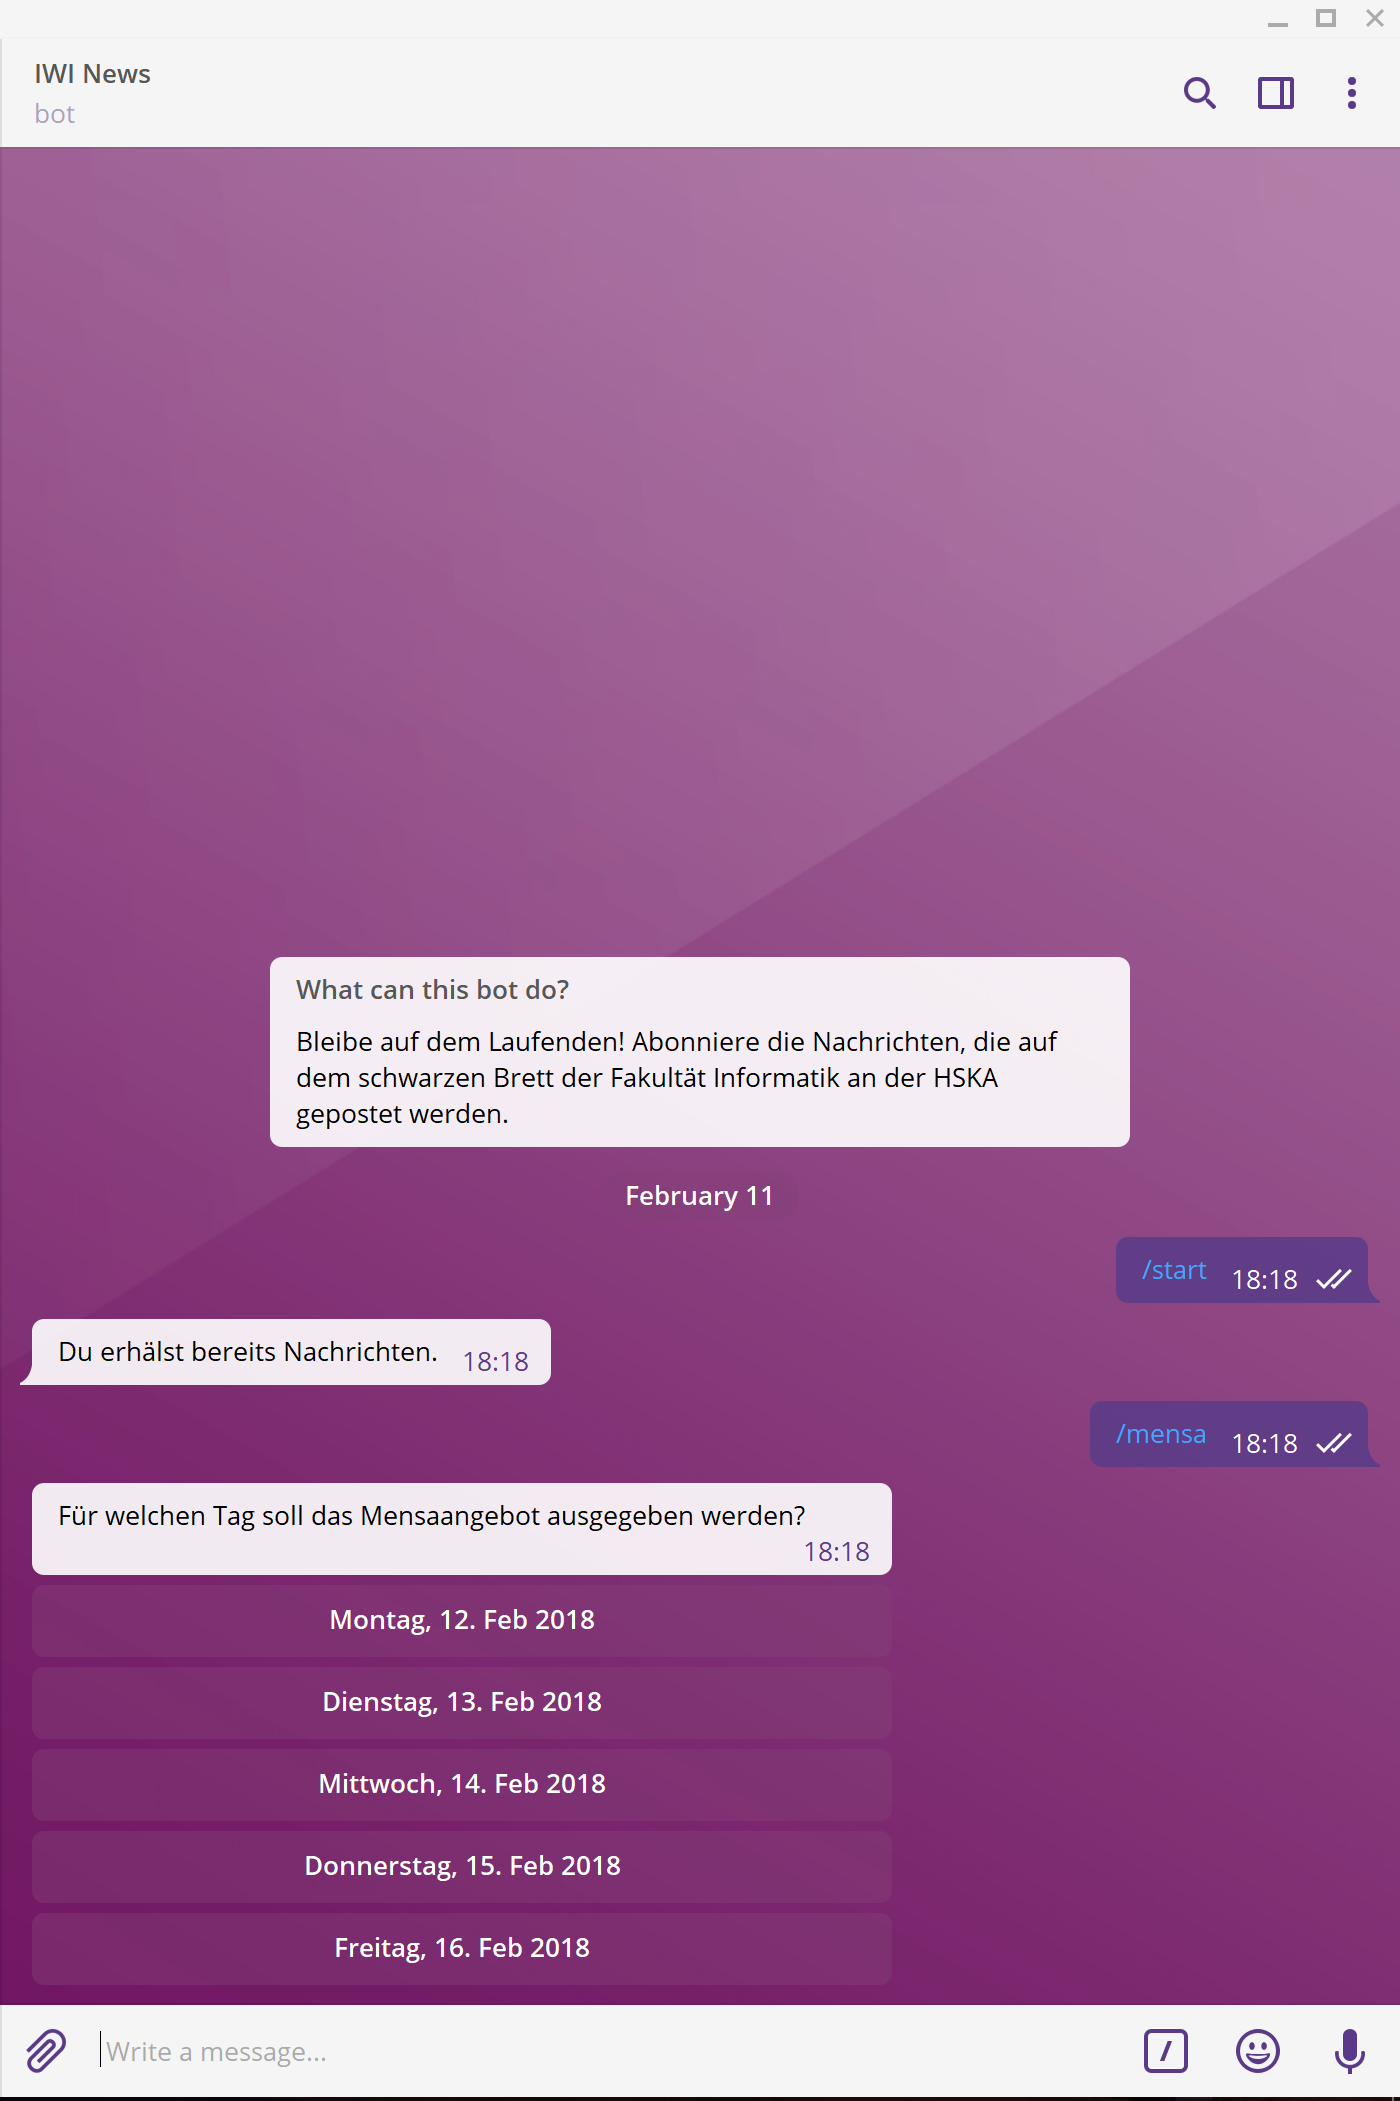
\includegraphics[width=0.4\linewidth]{BotMensa.png}
      \caption*{Quelle: Eigene Abbildung}
  \end{figure}
  \item[/settings] \hfill \\
  Der Benutzer kann zwischen verschiedenen Preisperspektiven auswählen: Mitarbeiter/Mitarbeiterinnen oder Studierende oder beides.
  \item[/profs] \hfill \\
  Der User erhält eine Liste aller Professoren/innen. Bei Klicken eines entsprechenden Buttons werden Informationen angezeigt. Darunter E-Mail-Adresse, wo das Büro des Lehrenden zu finden ist und wann die Sprechzeiten stattfinden.
  \item[/about] \hfill \\
  Tobias Kerst und Anna-Lena Schwarzkopf werden als Ansprechpartner für den Telegram-Bot während ihres Studiums gelistet.
\end{description}
